% vim:spelllang=ru,en
\documentclass[a4paper,12pt,notitlepage,headsepline,pdftex]{scrartcl}

\usepackage{cmap} % чтобы работал поиск по PDF
\usepackage[T2A]{fontenc}
\usepackage[utf8]{inputenc}
\usepackage[english,russian]{babel}
\usepackage{concrete}
\usepackage{cite}
\usepackage{url}

\usepackage{textcase}
\usepackage[pdftex]{graphicx}

\usepackage{lscape}

\pdfcompresslevel=9 % сжимать PDF
\usepackage{pdflscape} % для возможности альбомного размещения некоторых страниц
\usepackage[pdftex]{hyperref}
% настройка ссылок в оглавлении для pdf формата
\hypersetup{unicode=true,
            pdftitle={ПОЭВМ Лаба №2},
            pdfauthor={Погода Михаил},
            pdfcreator={pdflatex},
            pdfsubject={},
            pdfborder    = {0 0 0},
            bookmarksopen,
            bookmarksnumbered,
            bookmarksopenlevel = 2,
            pdfkeywords={},
            colorlinks=true, % установка цвета ссылок в оглавлении
            citecolor=black,
            filecolor=black,
            linkcolor=black,
            urlcolor=blue}

\usepackage{amsmath}
\usepackage{amssymb}
\usepackage{moreverb}
\usepackage{indentfirst}
\usepackage{misccorr}

\usepackage{xtab}
\usepackage{nccfoots}
\usepackage{listings}

\lstloadlanguages{C++}
\lstset{language=C++,basicstyle=\scriptsize,frame=tb,commentstyle=\itshape,stringstyle=\bfseries,extendedchars=false}
\begin{document}
\begin{titlepage}
  \begin{center}
    \large
    \MakeUppercase{Министерство образования и науки,}

    \MakeUppercase{молодёжи и спорта Украины}

    \mbox{\MakeUppercase{Национальный технический университет Украины}}

    \MakeUppercase{,,Киевский политехнический институт''}

    \addvspace{6pt}

    \normalsize
    Кафедра прикладной математики

    \vfill

    \textbf{Отчёт}

    Лабораторная работа \No 2

    по дисциплине ,,Программное обеспечение ЭВМ''

    \emph{,,Численное дифференцирование и интегрирование''}
  \end{center}

  \vfill

  \noindent
  \begin{minipage}{0.3\textwidth}
    Выполнил

    студент группы КМ-92

    Погода~М.\,В.
  \end{minipage}
  \hfill
  \begin{minipage}{0.4\textwidth}
    Проверила:

    Ковальчук"=Химюк~Л.\,А.
  \end{minipage}
  \vfill

  \begin{center}
    КИЕВ

    2012
  \end{center}
\end{titlepage}
\tableofcontents
\newpage
\section{Постановка задачи}
  Даны
  \begin{itemize}
    \item подынтегральная функция $f$~\eqref{eq:f};
    \item интервал интегрирования $\left[ a; b \right]$;
    \item шаг разбиения $h$;
    \item первообразная функция $F$~\eqref{eq:F}.
  \end{itemize}
  Необходимо найти на ЭВМ:
  \begin{itemize}
    \item Найти $\displaystyle\int_a^b f\left( x \right)\,dx$.
    \item Найти $\displaystyle\frac{dF\left( x \right)}{dx}$.
    \item Оценить точность полученных значений.
  \end{itemize}
\section{Входные данные}
  \hfill\emph{Вариант~11}

  \begin{itemize}
    \item Подынтегральная функция:
      \begin{equation}
        f = \frac{1}{x\sqrt{x^2 + 0.25}}
        \label{eq:f}
      \end{equation}
    \item Интервал интегрирования: $\left[ 1.0; 2.0 \right]$.
    \item Шаг разбиения $h = 0.02$.
    \item Первообразная функция:
      \begin{equation}
        F = -2\ln\frac{0.5 + \sqrt{x^2 + 0.25}}{x}
        \label{eq:F}
      \end{equation}
  \end{itemize}

  Метод численного интегрирования --- метод средних (центральных)
  прямоугольников.
  \newpage
\section{Теоретические сведения}
  Метод прямоугольников --- самый простой метод численного интегрирования,
  который заключается в замене значений функции на интервале на какое-то
  значение функции из этого интервала.

  Формула средних (центральных) прямоугольников:
  \begin{equation}
    \int_a^b f\left( x \right)\,dx = \left( b - a \right)f\left( \frac{a+b}{2}
    \right)
    \label{eq:cab}
  \end{equation}

  Производная --- основное понятие дифференциального исчисления, которое
  характеризует скорость изменения функции.
  Определяется как граница отношения прироста функции к приросту аргумента,
  когда аргумент стремится к нулю:
  \begin{equation}
    \frac{dF\left( x \right)}{dx} = \lim_{\Delta x \to 0}\frac{F\left( x +
    \Delta x \right) - F\left( x \right)}{\Delta x}
    \label{eq:diff}
  \end{equation}

  Для численного поиска производной можно воспользоваться формулой:
  \begin{equation}
    \frac{dF\left( x \right)}{dx} = \frac{F\left( x + h \right) - F\left(
    x \right)}{h}
    \label{eq:ndiff}
  \end{equation}
  \newpage
\section{Решение}
  \subsection{Значение интеграла, полученное численным методом}
    \begin{equation}
      I = 0.467
      \label{eq:I}
    \end{equation}
  \subsection{Проверка полученного значения интеграла}
    Для проверки полученного значения интеграла можно воспользоваться формулой
    Ньютона"=Лейбница:
    \begin{equation}
      \int_a^b f\left( x \right)\,dx = F\left( b \right) - F\left( a
      \right) = 0.467
      \label{eq:NL}
    \end{equation}

    Абсолютная погрешность: $\Delta I = 2.29\cdot10^{-5}$
  \subsection{Численное дифференцирование и оценка полученного результата}
    График производной и график, полученный численным дифференцированием
    приведён на снимке экранной формы в Приложении на
    странице~\pageref{fig:gui}.

\section{Описание программы}
  Программа написана на языке C++ с использованием библиотек
  Qt\footnote{\url{http://qt-project.org}} и
  Qwt\footnote{\url{http://qwt.sourceforge.net}}.

  Программа считает интеграл/производную от функций, заданных в условии,
  позволяя изменить приделы интегрирования и количество интервалов разбиения.

  В результате работы программы выводит на форме значение интеграла,
  полученного численным методом, значение интеграла, полученное по формуле
  Ньютона"=Лейбница, абсолютную погрешность вычислений, а также графики
  функции и производной первообразной, полученной численным методом.
  \newpage
\section{Блок"=схема алгоритма}
  \begin{figure}[h!]
    \begin{center}
      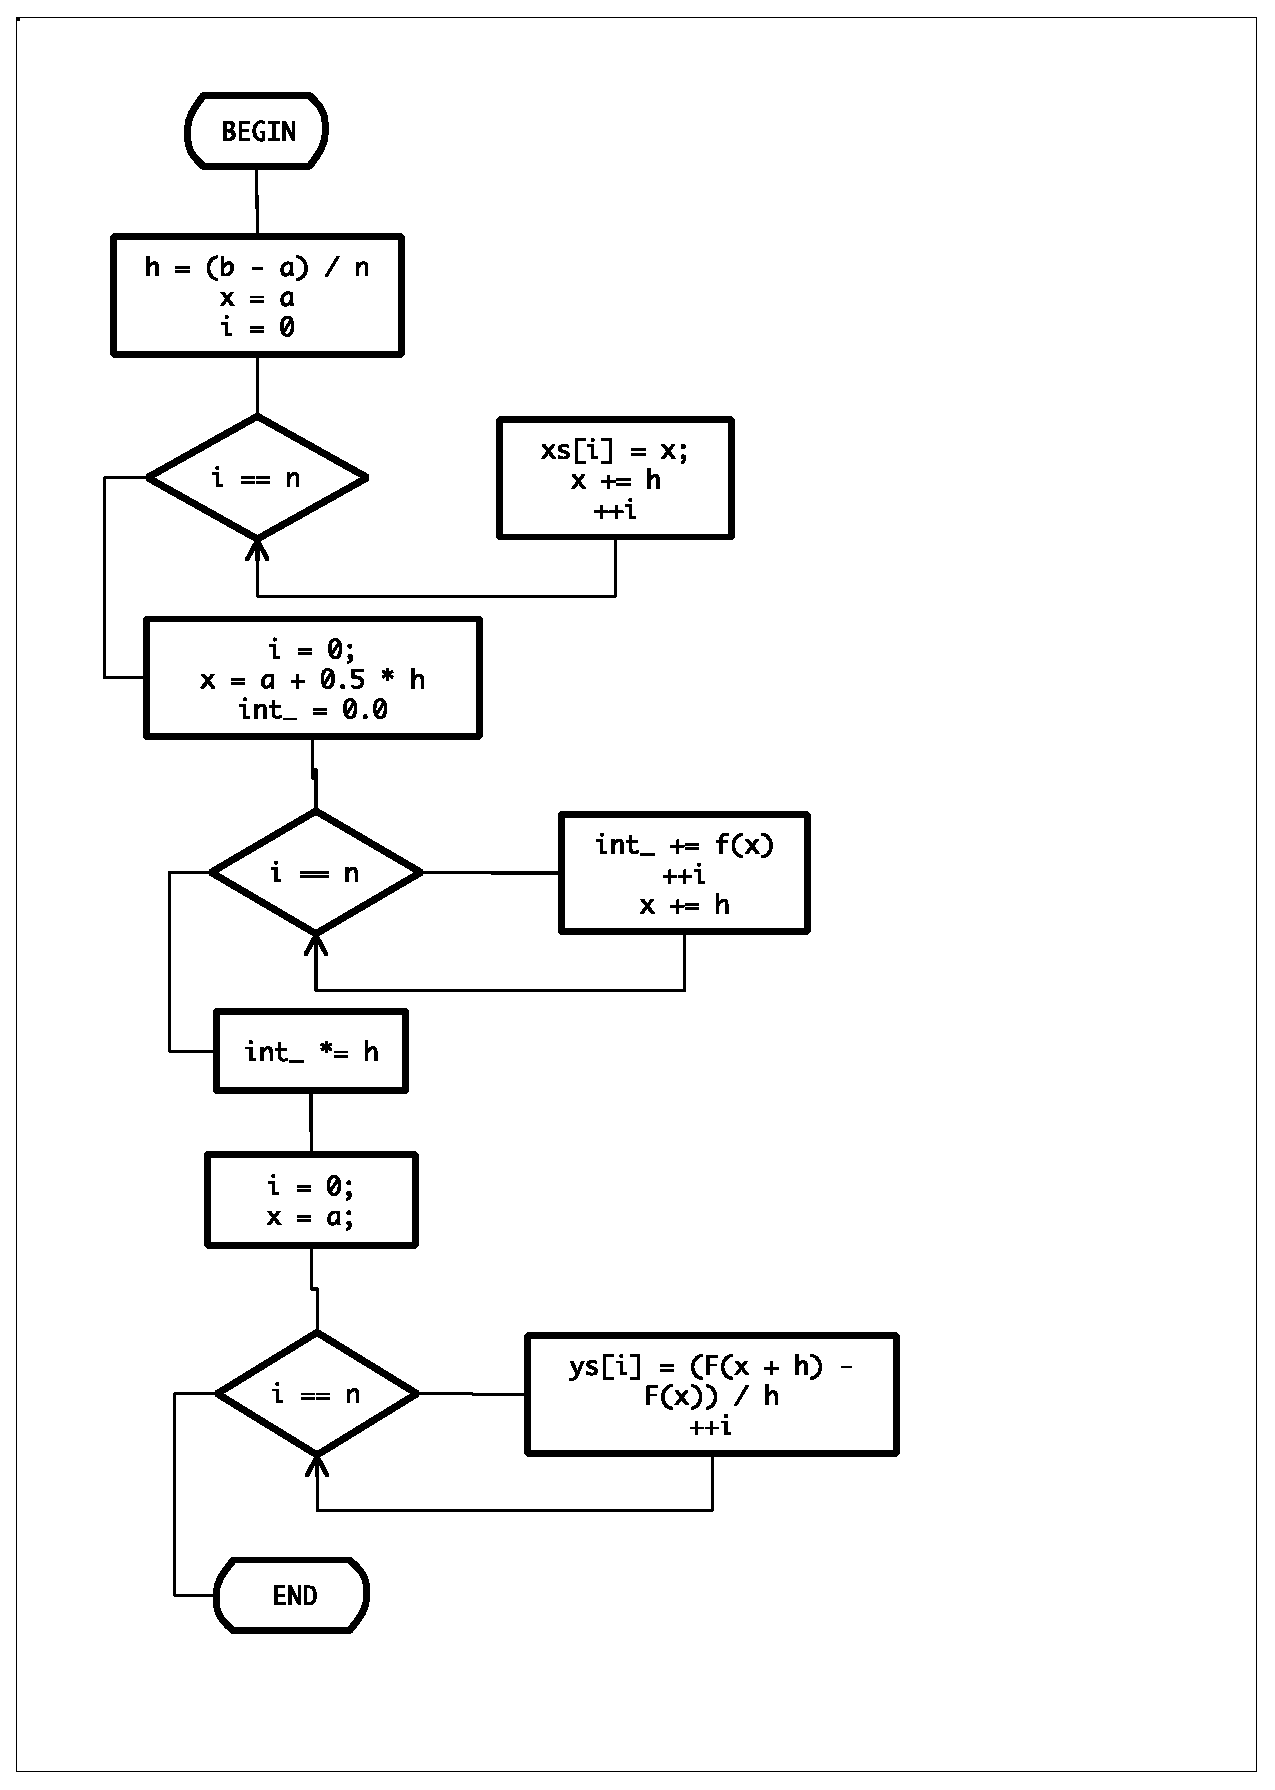
\includegraphics[scale=0.60]{flowchart.eps}
    \end{center}
    \caption{Блок"=схема алгоритма}
    \label{fig:flowchart}
  \end{figure}
  \newpage
\section{Выводы}
  При выполнении данной лабораторной работы был реализован метод вычисления
  определённого интеграла по формуле средних (центральных) прямоугольников, а
  также проверка полученного значения по формуле Ньютона"=Лейбница.
  Абсолютная погрешность составила $\approx 10^{-5}$ при данном шаге (0.2),
  поэтому можно утверждать, что этот метод показывает довольно неплохие
  результаты при достаточно маленьком шаге.
  При уменьшении шага точность, разумеется, увеличивается.

  Также были найдены значения производной первообразной в точках разбиения и
  построен график, на котором были отображены как эти значения, так и значения
  функции в этих точках.
  Из этого сравнительного графика видно, что производная, вычисленная
  численным методом, имеет погрешность $~2--3\%$ относительно реального
  значения.
  \newpage
\section{Приложения}
  \subsection{Графическая форма приложения}
    \begin{figure}[h!]
      \begin{center}
        \includegraphics[scale=0.86]{scr.png}
      \end{center}
      \caption{Графическая форма приложения}
      \label{fig:gui}
    \end{figure}
  \subsection{Исходные тексты}
    \subsubsection{CMakeLists.txt}
      \lstinputlisting{/home/projects/apps-for-computing/lab2/CMakeLists.txt}
    \subsubsection{lab2\_widget.hxx}
      \lstinputlisting{/home/projects/apps-for-computing/lab2/lab2_widget.hxx}
    \subsubsection{lab2\_widget.cxx}
      \lstinputlisting{/home/projects/apps-for-computing/lab2/lab2_widget.cxx}
\end{document}
